\chapter{Iterative Methods}


\section{Root finding problems}

\subsection{Incremental Search Method}

The approximate locations of the roots are best determined by plotting the function.
Often a very rough plot, based on a few points, is sufficient to provide reasonable
starting values.

The basic thought behind the incremental search method is simple:
If $ f(x_1) $ and $ f(x_2) $ have opposite signs, then there is at least one root
in the interval $ (x_1, x_2) $. If the interval is small enough, it is likely to
contain a single root. Thus the zeros of $ f(x) $ can be detected by evaluating the
function $ f(x) $ at intervals $ \Delta x $ and looking for a change in sign.

There are several potential problems with the incremental search method:

\begin{itemize}
    \item It is possible to miss two closely spaced roots if the search increment
        $ \Delta x $ is larger than the spacing of the roots

    \item A double root (two roots that coincide) will not be detected.

    \item Certain singularities (poles) of $ f(x) $ can be mistaken for roots.
        For example, $ f(x) = tan(x) $ changes sign at $ x \pm \frac{1}{2} n \pi $,
        $ n = 1, 3, 5, \dots $. However, these locations are not true zeroes, because the
        function does not cross the x-axis.

\end{itemize}


\textbf{Example of incremental function in python:}

\begin{python}
import math

def rootsearch(f: object, a: float, b: float, dx: float) -> float:
    """function using incremental search on the interval <a, b>, in increments
    of dx, to find the bounds <x1, x2> of the smallest root of f(x).

    Args:
        f (object): function to find the smallest root of
        a (float):  lower bound of the search region
        b (float):  upper bound of the search region
        dx (float): search step

    Returns:
        x1 = x2 = None if no roots were detected.
        x1 < x2 = the bounds specified by dx (x2 = x1 + dx)
    """
    x1, f1 = a, f(a)
    x2, f2 = b, f(b)
    while math.sign(f1) == math.sign(f2):
        if x1 >= b:
            return None, None
        x1, f1 = x2, f2
        x2, f2 = x2 + dx, f(x2 + dx)
    else:
        return x1, x3

\end{python}


\subsection{Bisection Method}

After a root $ f(x) = 0 $ has been bracketed in the interval $ <x_1, x_2> $, several methods
can be used to close in on it. The method of \textbf{bisection} accomplishes it
by \textit{halving} the interval until the error is sufficiently small:

\begin{eqarray}
    \varepsilon_{err} &= \left| x_2 - x_1 \right| \\
    \varepsilon_{err} &\le \varepsilon_{tol} \\
\end{eqarray}

The method of \textbf{bisection} uses the same principle as the \textbf{incremental}
search method. If there is a root $ f(x) = 0 $ in the interval $ x \in <x_1, x_2> $ then:

\begin{equation}
    sign(f(x_1)) \ne sign(f(x_2))
\end{equation}

To halve the interval, we compute $ f(x_3) $, where $ x_3 = \frac{1}{2} \left( x_1 + x_2 \right) $
is the midpoint of the interval. If $ sign(f(x_3)) \ne sign(f(x_2)) $, then the root
must be in the interval $ <x_3, x_2> $ and we replace the $ x_1 $ by $ x_3 $. Otherwise
the root must be in the interval $ <x_1, x_3> $ and we replace thr $ x_2 $ by $ x_3 $.
In either case the interval is \textbf{halved}. The bisection is repeated until
the interval has been reduced such that $ \varepsilon_{err} \le \varepsilon_{tol} $.

It is easy to compute the number of bisections needed to reach the prescribed $ \varepsilon_{tol} $.
The original interval $ \Delta x $ is reduced to $ \Delta x / 2 $ after one bisection,
$ \Delta x / 2^2 $ after two bisections, and after $ n $ bisections it is
$ \Delta x/2^n $. Setting $ \Delta x / 2^n = \varepsilon $ and solving for $ n $, we get:

\begin{equation}
    n = \frac{\ln{ \left( \Delta x / \varepsilon \right) } }
             {\ln 2}
\end{equation}

Since $ n $ must be an integer, the ceiling of $ n $ is used (smalles integer greater $ n $).

\newpage
\textbf{Python implementation:}

\begin{python}
import math

def bisection(f: callable, x1: float, x2: float,
              deny_increase: bool = True, tol: float = 1.E-09) -> float:
    """Root finding algorithm using a bisection method. The root must be bracketed in
    (x1, x2).

    Args:
        f (callable):         reference to the function to evaluate
        x1 (float):           lower bounds of the root bracket
        x2 (float):           upper bounds of the root bracket
        deny_increase (bool): returns None if |f(x)| increases upon bisection
                              (default = False)
        tol (float):          allowed tolerance for root finding
                              (default = 1.0E-09)

    Returns:
        (float): if root has been found
        None:    otherwise

    Raises:
        ValueError: The root has not been bracketed.
    """
    f1 = f(x1)
    if f1 == 0.: # jackpot -> no more searching
        return x1

    f2 = f(x2)
    if f2 == 0.: # jackpot -> no more searching
        return x2

    if math.sign(f1) == math.sign(f2):
        raise ValueError(f"The root has not been bracketed in <{x1:f}, {x2:f}>.")

    n = int(math.ceil(math.log(abs(x2 - x1) / tol) / math.log(2.)))

    # the bisection itself
    for i in range(n):
        x3 = 0.5 * (x1 + x2)
        f3 = f(x3)
        # abs value of f(x) is larger than before
        if deny_increase and ((abs(f3) > abs(f1)) or (abs(f3) > abs(f2))):
            return None
        if f3 == 0.: # jackpot -> no more searching
            return x3
        elif math.sign(f3) != math.sign(f2):
            x1, f1 = x3, f3
        else:
            x2, f2 = x3, f3

    # return the midpoint of the resulting span
    return 0.5 * (x1 + x2)

\end{python}


\subsection{Methods Based on Linear Interpolation}

\subsubsection{Secant and False Position Methods}

The \textbf{secant} and \textbf{false position} methods are closely related.
Both methods require two starting estimates of the root, say $ x_1 $ and $ x_2 $.
The function $ f(x) $ is assumed to be approximately linear near the root, so
that the improved value $ x_3 $ of the root can be estimated by linear interpolation
between $ x_1 $ and $ x_2 $.

This yields the relationship:

\begin{equation}
    \frac{f_2}{x_3 - x_2} = \frac{f_1 - f_2}{x_2 - x_1}
\end{equation}

where the notation $ f_i = f(x_i) $ is used. Thus the improved estimate of the
root is:

\begin{equation}
    x_3 = x_2 - f_2 \frac{x_2 - x_1}{f_2 - f_1}
\end{equation}

The difference between \textbf{false position} and \textbf{secant} method is in
the manner the new estimate is dealt with.

\begin{itemize}
    \item The \textbf{false position} method is similar to the \textbf{bisection} method where
        it is necessary that the root is \textbf{bracketed} by $ x \in <x_1, x_2> $.
        When a new estimate $ x_3 $ is obtained, then if $ sign(f_3) = sign(f_1) $,
        we let $ x_1 \leftarrow x_3 $, otherwise we let $ x_2 \leftarrow x_3 $.
        In this manner, the root is always bracketed in $ <x_1, x_2> $.
        Then we run a new iteration until convergence criteria are met.

    \item The \textbf{secant} method is different in two ways. It does not require prior
        bracketing of the root, and it discards the oldest prior estimate of the
        root (i.e. after $ x_3 $ is computed, we let $ x_1 \leftarrow x_2 \leftarrow x_3 $).

\end{itemize}

The convergence of the \textbf{secant} method is \textbf{superlinear}, with the
error behaving as $ E_{k+1} = c E_{k}^{1.618} $, where the exponent 1.618... is called
the "golden ratio".

\newpage
\textbf{Python implementation of the secant method:}

\begin{python}
import math

def secant(f: callable, x1: float, x2: float,
           tol: float = 1.E-09, maxiter: int = 1000) -> float:
    """Root finding algorithm using a secant method.

    Args:
        f (callable):  reference to the function to evaluate
        x1 (float):    lower bounds of the root bracket
        x2 (float):    upper bounds of the root bracket
        tol (float):   allowed tolerance for root finding
                       (default = 1.0E-09)
        maxiter (int): maximum number of iterations allowed (default = 1000)

    Returns:
        (float): if root has been found

    Raises:
        ValueError: No convergence is achievable as (f1 == f2, function is constant)
        ValueError: Maximum number of iterations reached.
    """
    f1 = f(x1)
    if f1 == 0.: # jackpot -> no more searching
        return x1

    f2 = f(x2)
    if f2 == 0.: # jackpot -> no more searching
        return x2

    # the secant method itself
    for i in range(maxiter):
        if f1 == f2:
            raise ValueError(f"The function is constant in interval ({x1:f}, {x2:f}).")
        x3 = x2 - f2 * (x2 - x1) / (f2 - f1)
        f3 = f(x3)
        if f3 == 0.: # jackpot -> no more searching
            return x3
        elif abs(f3) <= tol:
            return x3
        else:
            # discard x1 and f1
            x1, f1, x2, f2 = x2, f2, x3, f3
    else:
        raise ValueError(f"Maximum number of iterations ({maxiter:d}) reached!")


\end{python}


\newpage
\subsubsection{Ridder's Method}

\textbf{Ridder's} method is a clever modification of the \textbf{false position}
method. Assuming ht root is bracketed in $ <x_1, x_2> $, whe first compute
$ f_3 = f(x_3) $, where $ x_3 $ is the midpoint of the bracket.

It can be noted:

\begin{eqarray}
    x_3 &= \frac{1}{2} \left( x_1 + x_2 \right) \\
    h &= \frac{1}{2} \left( x_2 - x_1 \right) \\
    \label{eqn:ridder_h}
\end{eqarray}

Next we introduce a new function $ g(x) $ such, that:

\begin{equation}
    \label{eqn:ridder_gx}
    g(x) = f(x) e^{\left( x - x_1 \right) Q}
\end{equation}

where the constant $ Q $ is determined by requiring the points $ (x_1, g_1) $,
$ (x_2, g_2) $ and $ (x_3, g_3) $ to lie on a straight line. As before, the
notation is $ g_i = g(x_i) $. The improved value $ x_4 $ is then obtained by
linear interpolation of $ g(x) $ rather than $ f(x) $.

From \ref{eqn:ridder_gx} we obtain:

\begin{eqarray}
    \label{eqn:ridder_gi}
    g_1 &= f_1 \\
    g_2 &= f_2 e^{2hQ} \\
    g_3 &= f_3 e^{hQ} \\
\end{eqarray}

where $ h $ is obtained from \ref{eqn:ridder_h}.

Using the requirement thet the three points $ g_1 $, $ g_2 $ and $ g_3 $ line on
straight line or:

\begin{equation}
    g_3 = \frac{g_1 + g_2}{2}
\end{equation}

or:

\begin{equation}
    f_3 e^{hQ} = \frac{1}{2} \left( f_1 + f_2 e^{2hQ} \right)
\end{equation}

which is a quadratic equation in $ e^{hQ} $. The solution is

\begin{lequation}[eqn:ridder_root]
    e^{hQ} = \frac{f_3 \pm \sqrt{f_3^2 - f_1 f_2 }}{f_2}
\end{lequation}

Linear interpolation based on points $ (x_1, g_1) $ and $ (x_3, g_3) $ now yields
for the improved root:

\begin{eqarray}
    x_4 &= x_3 - g_3 \frac{x_3 - x_1}{g_3 - g_1} \\
    x_4 &= x_3 - f_3 e^{hQ} \frac{x_3 - x_1}{f_3 e^{hQ} - f_1} \\
\end{eqarray}

where in the last step the \ref{eqn:ridder_gi} is used. As the final step,
a substitution for $ e^{hQ} $ is used from \ref{eqn:ridder_root} and after
some algebra the following solution is obtained:

\begin{lequation}[eqn:ridder_x4]
    x_4 = x_3 \pm \left( x_3 - x_1 \right) \frac{f_3}{\sqrt{f_3^2 - f_1 f_2}}
\end{lequation}

it can be shown that the correct result is obtained by choosing the $ + $ sign
if $ f_1 - f_2 > 0 $ and the minus signe if $ f_1 - f_2 < 0 $.

The \ref{eqn:ridder_x4} can be then adjusted as:

\begin{lequation}[eqn:ridder_x4_sign]
    x_4 = x_3 + sign \left( f_1 - f_2 \right) \times \left( x_3 - x_1 \right) \frac{f_3}{\sqrt{f_3^2 - f_1 f_2}}
\end{lequation}

After the computation of $ x_4 $, new brackets are determined for the root and
\ref{eqn:ridder_x4_sign} is applied again. The procedure is repeated until the
difference between two successive values of $ x_4 $ becomes negligible.

The \textbf{Ridder's} iterative formula in \ref{eqn:ridder_x4_sign} has a very
useful property: If $ x_1 $ and $ x_2 $ bracket the root, then $ x_4 \in <x_1, x_2> $
in all cases. In other words, once the root is bracketed, it stays bracketed.

\textbf{Ridder's} method can be shown to converge \textbf{quadratically}, making
it faster than either the \textbf{secant} or the \textbf{false position} method.

\begin{bbox}
\textbf{It is the method to use if the derivative of $ f(x) $ is impossible or
difficult to compute.}
\end{bbox}


\newpage
\textbf{Python implementation:}

\begin{python}
import math

def ridder(f: callable, x1: float, x2: float,
           rtol: float = 1.E-09, maxiter: int = 1000) -> float:
    """Root finding algorithm using a Ridder's algorithm. The root must be
    bracketed in (x1, x2).

    Args:
        f (callable):  reference to the function to evaluate
        x1 (float):    lower bounds of the root bracket
        x2 (float):    upper bounds of the root bracket
        tol (float):   allowed tolerance for root finding
                       absolute for found root, relative for
                       change between root iteraions
                       (default = 1.0E-09)
        maxiter (int): maximum number of iterations
                       (default = 1000)

    Returns:
        (float): if root has been found
        None:    if root is not bracketed

    Raises:
        ValueError: Maximum number of iterations reached.
    """
    f1 = f(x1)
    if abs(f1) <= tol: # jackpot -> no more searching (absolute error)
        return x1

    f2 = f(x2)
    if abs(f2) <= tol: # jackpot -> no more searching (absolute error)
        return x2

    if math.sign(f1) == math.sign(f2):
        return None

    x3 = 0.5 * (x1 + x2)

    # the Ridder's method itself
    xold = x1
    for i in range(maxiter):
        x3 = (x1 + x2) / 2
        f3 = f(x3)
        if abs(f3) <= tol: # jackpot -> no more searching (absolute error)
            return x3
        s = math.sqrt(f_3 ** 2 - f_1 * f_2)
        if s == 0.:
            return None
        dx = (x3 - x1) * f3 / s
        x4 = x3 + math.sign(f1 - f2) * dx
        f4 = f(x4)
        if abs(f4) <= tol: # jackpot -> no more searching (absolute error)
            return x4

        # test for convergence -> relative error
        if abs(x4 - xold) <= tol * abs(x4):
            return x4
        xold = x4

        # Re-bracket the root as tightly as possible
        if math.sign(f3) == math.sign(f4):
            if math.sign(f1) != math.sign(f4):
                # f1  0  f4  f3  f2
                x2, f2 = x4, f4
            else:
                # f1  f3  f4  0  f2
                x1, f1 = x4, f4
        else:
            # f1  f3  0  f4  f2
            x1, f1, x2, f2 = x3, f3, x4, f4

    else:
        raise ValueError(f"Maximum number of iterations ({maxiter:d}) reached!")

\end{python}


\newpage
\subsubsection{Newton-Raphson Method}

The \textbf{Newton-Raphson} algorithm is the best known method of finding roots
for a good reason: it is \textbf{simple} and \textbf{fast}. The only drawback
of the method is that it uses the \textbf{derivative} $ f'(x) $ of the function
as well as the function $ f(x) $ itself. Therefore, the \textbf{Newton-Raphson}
method is usable only in problesm where $ f'(x) $ can be readily computed.

The \textbf{Newton-Raphson} formula can be derived from the \textbf{Taylor series}
expansion of $ f(x) $ about $ x $:

\begin{lequation}[eqn:newton-raphson_taylor]
    f(x_{i+1}) = f(x_i) + f'(x_i)(x_{i+1} - x_i) + \mathcal{O} (x_{i+1} - x_i)^2
\end{lequation}

where $ \mathcal{O}(z) $ is to be read as "of the order of $ z $". If $ x_{i+1} $ is
a root of $ f(x) = 0 $. The formula \ref{eqn:newton-raphson_taylor} becomes:

\begin{lequation}[eqn:newton-raphson_zero]
    0 = f(x_i) + f'(x_i)(x_{i+1} - x_i) + \mathcal{O} (x_{i+1} - x_i)^2
\end{lequation}

Assuming that $ x_i \to x_{i+1} $, we can dorp the last term
in \ref{eqn:newton-raphson_zero} and solve for $ x_{i+1} $.

\begin{bbox}
    Then the  \textbf{Newton-Raphson} formula is:

    \begin{lequation}[eqn:newton-raphson]
        x_{i+1} = x_i - \frac{f(x_i)}{f'(x_i)}
    \end{lequation}
\end{bbox}

The formula \ref{eqn:newton-raphson} appriximates $ f(x) $ by the straight line
that is tangent to the curve at $ x_i $. This $ x_{i+1} $ is at the intersection of
the x-axis and the tangent line.

\begin{bbox}
    The formula including $ f'(x_i) $ can be also derived using the following
    discrete approach (using $ \Delta $ as a finite neighborhood of $ x_i $):

    \begin{eqarray}
        f'(x_1) &= \frac{f(x_i + \Delta / 2) - f(x_i - \Delta / 2)}{(x_i + \Delta / 2) - (x_i - \Delta /2)} \\
        f'(x_1) &= \frac{f(x_i + \Delta / 2) - f(x_i - \Delta / 2)}{\Delta} \\
    \end{eqarray}

    then setting $ dx = \Delta $ and $ dy = f(x_i + \Delta / 2) - f(x_i - \Delta / 2) $:

    \begin{equation}
        f'(x_1) = \frac{dy}{dx}
    \end{equation}

    we can write:

    \begin{equation}
        x_{i+1} = x_i - dx \frac{f(x_i)}{dy}
    \end{equation}
\end{bbox}

The \textbf{algorithm} for the \textbf{Newton-Raphson} method is simple:

It repeatedly applies \ref{eqn:newton-raphson}, starting with an initial value
$ x_0 $, until convergence criterion $ \left| x_{i+1} - x_i \right| \le \varepsilon_{tol} $
is reached, the $ \varepsilon_{tol} $ being the error tolerance. Only the \textbf{latest}
value of $ x $ has to be stored.

\textbf{The algorithm is here:}
\begin{bbox}

    \begin{enumerate}
        \item Let $ x $ be an estimate of the root of $ f(x) = 0 $.

        \item Do until $ \left| \Delta x \right| \le \varepsilon_{tol} $:

            \begin{enumerate}
                \item Compute $ \Delta x = - f(x) / f'(x) $
                \item Let $ x \leftarrow x + \Delta x $

            \end{enumerate}
    \end{enumerate}
\end{bbox}

The truncation error $ E $ in the \textbf{Newton-Raphson} formula can be shown to
behave as

\begin{equation}
    E_{i+1} = - \frac{f''(x)}{2f'(x)}E_i^2
\end{equation}

where $ x $ is the \textbf{root}. This indicates that the method converges
\textit{quadratically} (the error is the square of the error in the previous step).
Consequently the number of significant figures is roughly doubled in every
iteration.

Althou the \textbf{Newton-Raphson} method converges fast near the root, its global
convergence characteristics are poor. The reasion is that the tangent line is
not always an acceptable approximation of the function. However, the method can be
made nearly fail-safe by \textbf{combining} it with \textbf{bisection}.

The following \textit{safe version} of the \textbf{Newton-Raphson} method assumes
that the root to be computed is initially bracketed in $ <x_1, x_2> $.
The midpoint of the bracket is used as the initial guess of the root. The brackets
are updated after each iteration. If a \textbf{Newton-Raphson} iteration does not
stay within the brackets, it is disregarded and replaced with bisection.
Because the \textbf{Newton-Raphson} method uses the function $ f(x) $ as well as its
derivative, function routines for both (denoted as $ f $ and $ df $) must be provided.

\textbf{Python implementation:}

\begin{python}
import math

def newtonRaphson(f: callable, df: callable, x: float,
                  tol: float = 1.E-09, maxiter: int = 1000) -> float:
    for i in range(maxiter):
        try:
            dx = - f(x) / df(x)
        except ZeroDivisionError as e:
            raise ValueError(f"Function derivation  f'(x = {x:f}) = 0")
        x += dx
        if abs(dx) <= tol * abs(x):
            return x

    else:
        raise ValueError(f"Maximum iteration number reached ({maxiter:d}).")

def newtonRaphsonImproved(f: callable, df: callable, x1: float, x2: float,
                          tol: float = 1.E-09, maxiter: int = 1000) -> float:
    f1 = f(x1)
    if abs(f1) <= tol:
        return x1

    f2 = f(x2)
    if abs(f2) <= tol:
        return x2

    if math.sign(f1) == math.sign(f2):
        raise ValueError(f"Root is not bracketed by ({x1:f}, {x2:f}).")

    x3 = (x1 + x2) / 2
    for i in range(maxiter):
        f3 = f(x3)
        if abs(f3) <= tol:
            return x3

        # tighten the brackets on the root
        if math.sign(f1) != math.sign(f3):
            x2 = x3
        else:
            x1 = x3

        # try a Newton-Raphson step
        df3 = df(x3)

        # if division by zero, push x3 out of bounds
        try:
            dx = -f3 / df3
        except ZeroDivisionError as e:
            dx = x2 - x1

        x3 += dx

        # if the result is out of brackets, use bisection
        if (x2 - x3) * (x3 - x1) < 0.:
            dx = (x2 - x1) / 2.
            x3 = x1 + dx

        # check for convergence
        if abs(dx) <= tol * abs(x2):
            return x3

    else:
        raise ValueError(f"Maximum iteration number reached ({maxiter:d}).")

\end{python}


\newpage
\section{Minimizing function of Multiple variables}

\subsubsection{Downhill Simplex Method}

\textbf{Downhill Simplex} method, also known as \textbf{Nelder-Mead} method
is best used when optimizing (finding of \textbf{minimum}) a function of
\textit{multiple} variables, especially when derivatives (the \textbf{Jacobian})
are hard or impossible to obtain.

The method is \textbf{robust} but \textbf{slow}. Special consideration must be
taken when preparing the function and when supplying constraints.

The \textbf{target function} to optimise usually takes the following form:

\begin{equation}
    S(\mathbf{x}) = F(\mathbf{x}) + \sum_{i=1}^{k} \lambda_i \left( T_i - C_i(\mathbf{x}) \right)^2
\end{equation}

where: \\
$ S(\mathbf{x}) $ is the optimised function \\
$ \mathbf{x} $ is a vector of variables $ \mathbf{x} = \left\{ x_1, x_2, \ldots , x_n \right\} $ \\
$ F(\mathbf{x}) $ is the function to optimise \\
$ T_i $ is the i-th constraint target value \\
$ C_i(\mathbf{x}) $ is the i-th constraint function, and \\
$ \lambda_i $ is the i-th constraint scaling weight factor, usually $ \lambda \gg 1.0 $.

The i-th constraint is $ \lambda_i \left(T_i - C_i(\mathbf{x}) \right)^2 $ which,
using the power of 2, is made to have higher weight the more the actual
$ C_i(\mathbf{x}) $ value differs from the constraint target $ T_i $ to both
sides of the spectra. The $ \lambda_i $ parameter is used to \textbf{scale}
the not yet met convergence criterion even further. It is especially effective
for values close to $ 0 $.

\begin{bbox}
    A \textbf{maximization} of a function $ F(\mathbf{x}) $ is actually equal to
    \textbf{minimization} of $ -F(\mathbf{x}) $.
\end{bbox}

The idea behind the \textbf{downhill simplex} method is to employ
a moving \textbf{simplex} in the design space to surround the optimal point and
then shrink the simplex until its dimensions reach the specified error of tolerance.
In $ n $-dimensional space a \textbf{simplex} is a figure of $ n + 1 $ vertices
connected by straight lines and bounded by polygonal faces. If $ n = 1 $,
a \textbf{simplex} is a line. If $ n = 2 $, a \textbf{simplex} is a triangle,
\textbf{tetrahedron} if $ n = 3 $.

\begin{figure}[ht]
    \begin{subfigure}[h]{0.6\linewidth}
        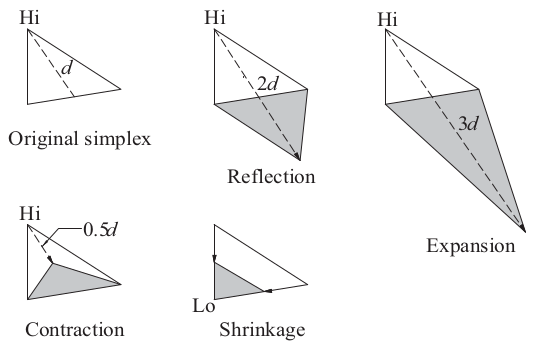
\includegraphics[width=\linewidth]{img/2dsimplex.png}
        \caption{Allowed moves for a 2D simplex}
        \label{fig:2dsimplex-png}
    \end{subfigure}
    \hfill
    \begin{subfigure}[h]{0.4\linewidth}
        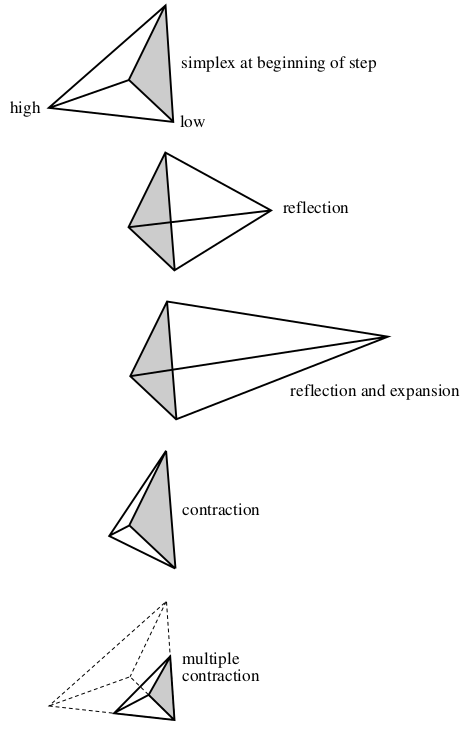
\includegraphics[width=\linewidth]{img/3dsimplex.png}
        \caption{Allowed moves for a 3D simplex}
        \label{fig:3dsimplex-png}
    \end{subfigure}
    \caption{Allowed simplex moves for $ n = 2 $ and $ n = 3 $}
    \label{fig:simplex-moves}
\end{figure}

The allowed moves of a \textbf{two-dimensional simplex} ($ n = 2 $) and
\textbf{three-dimensional simplex} ($ n = 3 $) are illustrated
on pictures \ref{fig:simplex-moves}.

By applying these moves in a suitable sequence,
the \textbf{simplex} can \textbf{always} hunt down the minimum point, enclose it,
and then shrink around it. The direction of a bove is determined by the values of
$ S(\mathbf{x}) $ (the function to be minimised, including constraints) at the
\textbf{vertices}. The vertex with the \textbf{highest} value of $ S $
is labeled $ Hi $, and $ Lo $ denotes the vertex with the \textbf{lowest} value.

The magnitude of a move is controlled by the distance $ d $ measured from the
$ Hi $ vertex to the \textbf{centroid} of the opposing vertices.

The \textbf{centroid} is simply an arithmetic average of the other vertices.

\begin{eqarray}
    x_{iHi} &= Hi \\
    x_c &= \sum_{i \ne i_{Hi}}^{n} x_{i} / \left( n - 1 \right) \\
    d &= x_c - x_{iHi} \\
\end{eqarray}

The outline of the algorithm is as follows:
\begin{bbox}

    \begin{itemize}
        \item Choose a starting simplex (using side parameter)
        \item Cycle until $ d \le \epsilon_{tol} $
        \begin{itemize}
            \item find \textbf{vertices} $ v_{Hi} $, $ v_{Lo} $ with the highest and lowest
                value of $ S(\mathbf{x}) $, respectively
            \item compute $ d = \left| v_{Hi} - \sum \left( v \ne v_{Hi} \right) / (n - 1) \right| $
            \item Try \textbf{reflection} $ v_n = v_{Hi} - 2d $
            \item if $ S(v_n) \le S(v_{Lo}) $: accept \textbf{reflection} $ v_{Hi} = v_n $

            \begin{itemize}
                \item Try \textbf{expansion}: $ v_n = v_n - d $

                \item if $ S(v_n) \le S(v_{Lo}) $: accept \textbf{expansion} $ v_{Hi} = v_n $

            \end{itemize}
            \item else:
            \begin{itemize}
                \item if $ S(v_n) \le S(v_{Hi}) $:
                \begin{itemize}
                    \item Try \textbf{contraction}: $ v_n = v_{Hi} - d / 2 $

                    \item if $ S(v_n) \le S(v_{Hi}) $: accept \textbf{contraction} $ v_{Hi} = v_n $

                \end{itemize}
                \item else: use \textbf{shrinkage}:
                    $ v_{i} = \left( v_{i} + v_{Hi} \right) / 2 \q \forall \q v_i \ne v_{Hi} $

            \end{itemize}
        \end{itemize}
    \end{itemize}

\end{bbox}

The \textbf{downhill simplex method} is much slower than other methods in most
cases, but makes up for it in robustness. It often works for problems where
other methods hang up.

The starting simplex for a three parameter optimization (with $ \delta $ side parameter):

\begin{eqarray}
    \mathbf{x_0} &= \left\{ x_1, x_2, x_3 \right\} \\
    \mathbf{x} &= \begin{bmatrix}
        x_1 & x_2 & x_3 \\
        x_1 + \delta & x_2 & x_3 \\
        x_1 & x_2 + \delta & x_3 \\
        x_1 & x_2 & x_3 + \delta \\
        \end{bmatrix} \\
\end{eqarray}


\textbf{Python implementation:}

\begin{python}
import numpy as np
import math

def downhill(F: callable, x0: np.ndarray,
     side: float = 0.1, tol: float = 1.0e-6, maxiter: int = 500,
     ro: float = 1.0, epsilon: float = 2.,
     gamma: float = 0.5, sigma: float = 0.5) -> np.ndarray:
    '''Downhill simplex method for minimization (Nelder-Mead method)

    Args:
        F (callable):    reference to scalar function that should be minimized
        x0 (np.ndarray): starting vector x = initial estimate
        side (float):    side length of the starting simplex (default = 0.1)
        tol (float):     convergence toelerance (default = 1.0e-06)
        maxiter (int):   maximum number of iterations (default = 500)
        ro (float):      reflection coefficient   (default ro      = 1.0)
        epsilon (float): expansion coefficient    (default epsilon = 2.0)
        gamma (float):   contraction coefficient  (default gamma   = 0.5)
        sigma (float):   shrink coefficient       (default sigma   = 0.5)

    Returns:
        (np.ndarray): the optimized values

    '''
    n = len(x0) # Number of variables

    # Generate starting simplex
    x = np.repeat(x0.reshape(1,-1), repeats=n+1, axis=0)
    # move each parameter by 'side'
    x[1:,:] += np.eye(n, n) * side

    # Compute values of F at the vertices of the simplex
    f = np.apply_along_axis(F, axis=1, arr=x)

    # Main loop
    for k in range(maxiter):
        # Sort vertices from lowest to highest (indexes: lowest = 0, highest = n)
        idx = np.argsort(f)
        f, x = f[idx], x[idx]

        # The centroid of all vertices except the highest xcog = sum x(i<n) / n
        # Compute the move vector d (from highest vertex to centroid of rest)
        # d = xcog - xn
        d = np.sum(x[:-1], axis=0) / n - x[-1]

        # Check for convergence
        if math.sqrt(np.dot(d, d) / n) < tol:
            print(f"[+] Convergence reached at iteration: {k:d}")
            return x[0]

        # Try reflection: xr = xcog + ro * (xcog - xn)
        xNew = x[-1] + (1.0 + ro) * d
        fNew = F(xNew)
        if fNew <= f[0]: # Accept reflection
            x[-1], f[-1] = xNew, fNew

            # Try expanding the reflection: xe = xcog + epsilon * (xr - xcog)
            xNew = x[-1] + (epsilon - ro) * d
            fNew = F(xNew)

            if fNew <= f[0]: # Accept expansion
                x[-1], f[-1] = xNew, fNew

        # Try reflection again
        elif fNew <= f[-1]: # Accept reflection
            x[-1], f[-1] = xNew, fNew

        else:
            # Try contraction: xc = xcog + gamma * (xr - xcog)
            xNew = x[-1] + gamma * d
            fNew = F(xNew)

            if fNew <= f[-1]: # Accept contraction
                x[-1], f[-1] = xNew, fNew

            else:
                # Use shrinkage: xi = xi + sigma * (xi - x0)
                x[1:] += sigma * (x[1:] - x[0])
                f[1:] = np.apply_along_axis(F, axis=1, arr=x[1:])

    print(f"[-] Iteration limit exceeded: {maxiter:d}")
    return x[0]

\end{python}




\newpage
\section{second order ODE's}

Most of FEM problems are \textbf{second order Ordinary Differential Equations}, e.g:

\begin{eqarray}
    m \frac{u''(t)}{d^2 t} + c \frac{u'(t)}{dt} + k u(t) &= 0\\
    m \ddot{u} + c \dot{u} + k u &= 0\\
    m a + c v + ku &= 0
\end{eqarray}

while the iterative methods are for \textbf{first order ODE's} only.
A \textbf{substitution} technique is therefore used to transform the
\textbf{second order ODE's} to a set of \textbf{first order ODE's} and these are
then solved sequentialy.

First we begin with a \textbf{second order ODE} in the form of:

\begin{equation}
    a \frac{y''(x)}{d^2 x} + b \frac{y'(x)}{dx} + c y = d, \quad with \quad y(0) = y_0 \quad and \quad
    \frac{y'(0)}{dx} = y_1
\end{equation}

By stating:

\begin{equation}
    \frac{dy}{dx} = z
\end{equation}

and substituting back:

\begin{equation}
    a \frac{dz}{dx} + b z + c y = d
\end{equation}

now we can write the following set of equations:

\begin{eqarray}
    \begin{aligned}
        z &= \frac{dy}{dx}\\
        \frac{dz}{dx} &= \frac{d - c y - b z}{a}
    \end{aligned} &
    \quad \left\{
    \begin{aligned}
        y(0) &= y_0\\
        z(0) &= y_1
    \end{aligned} \right.
\end{eqarray}



\section{Explicit}

\subsection{Euler's method}
The \textbf{Euler's Method} is an iterative method to solve ODEs. This method's
huge plus is it is fast. The minus is it gradually diverges from the ideal solution.

The \textbf{Euler's Method} uses the following formula:

\begin{equation}
    y(t + h) = y(t) + h f(x,y)
\end{equation}

to construct the tangent at point $ x $ and obtain the value of $ y(x + h) $,
whose slope is:

\begin{equation}
    f(x,y) \quad or \quad \frac{dy}{dx}
\end{equation}

\begin{figure}[ht]
    \centering
    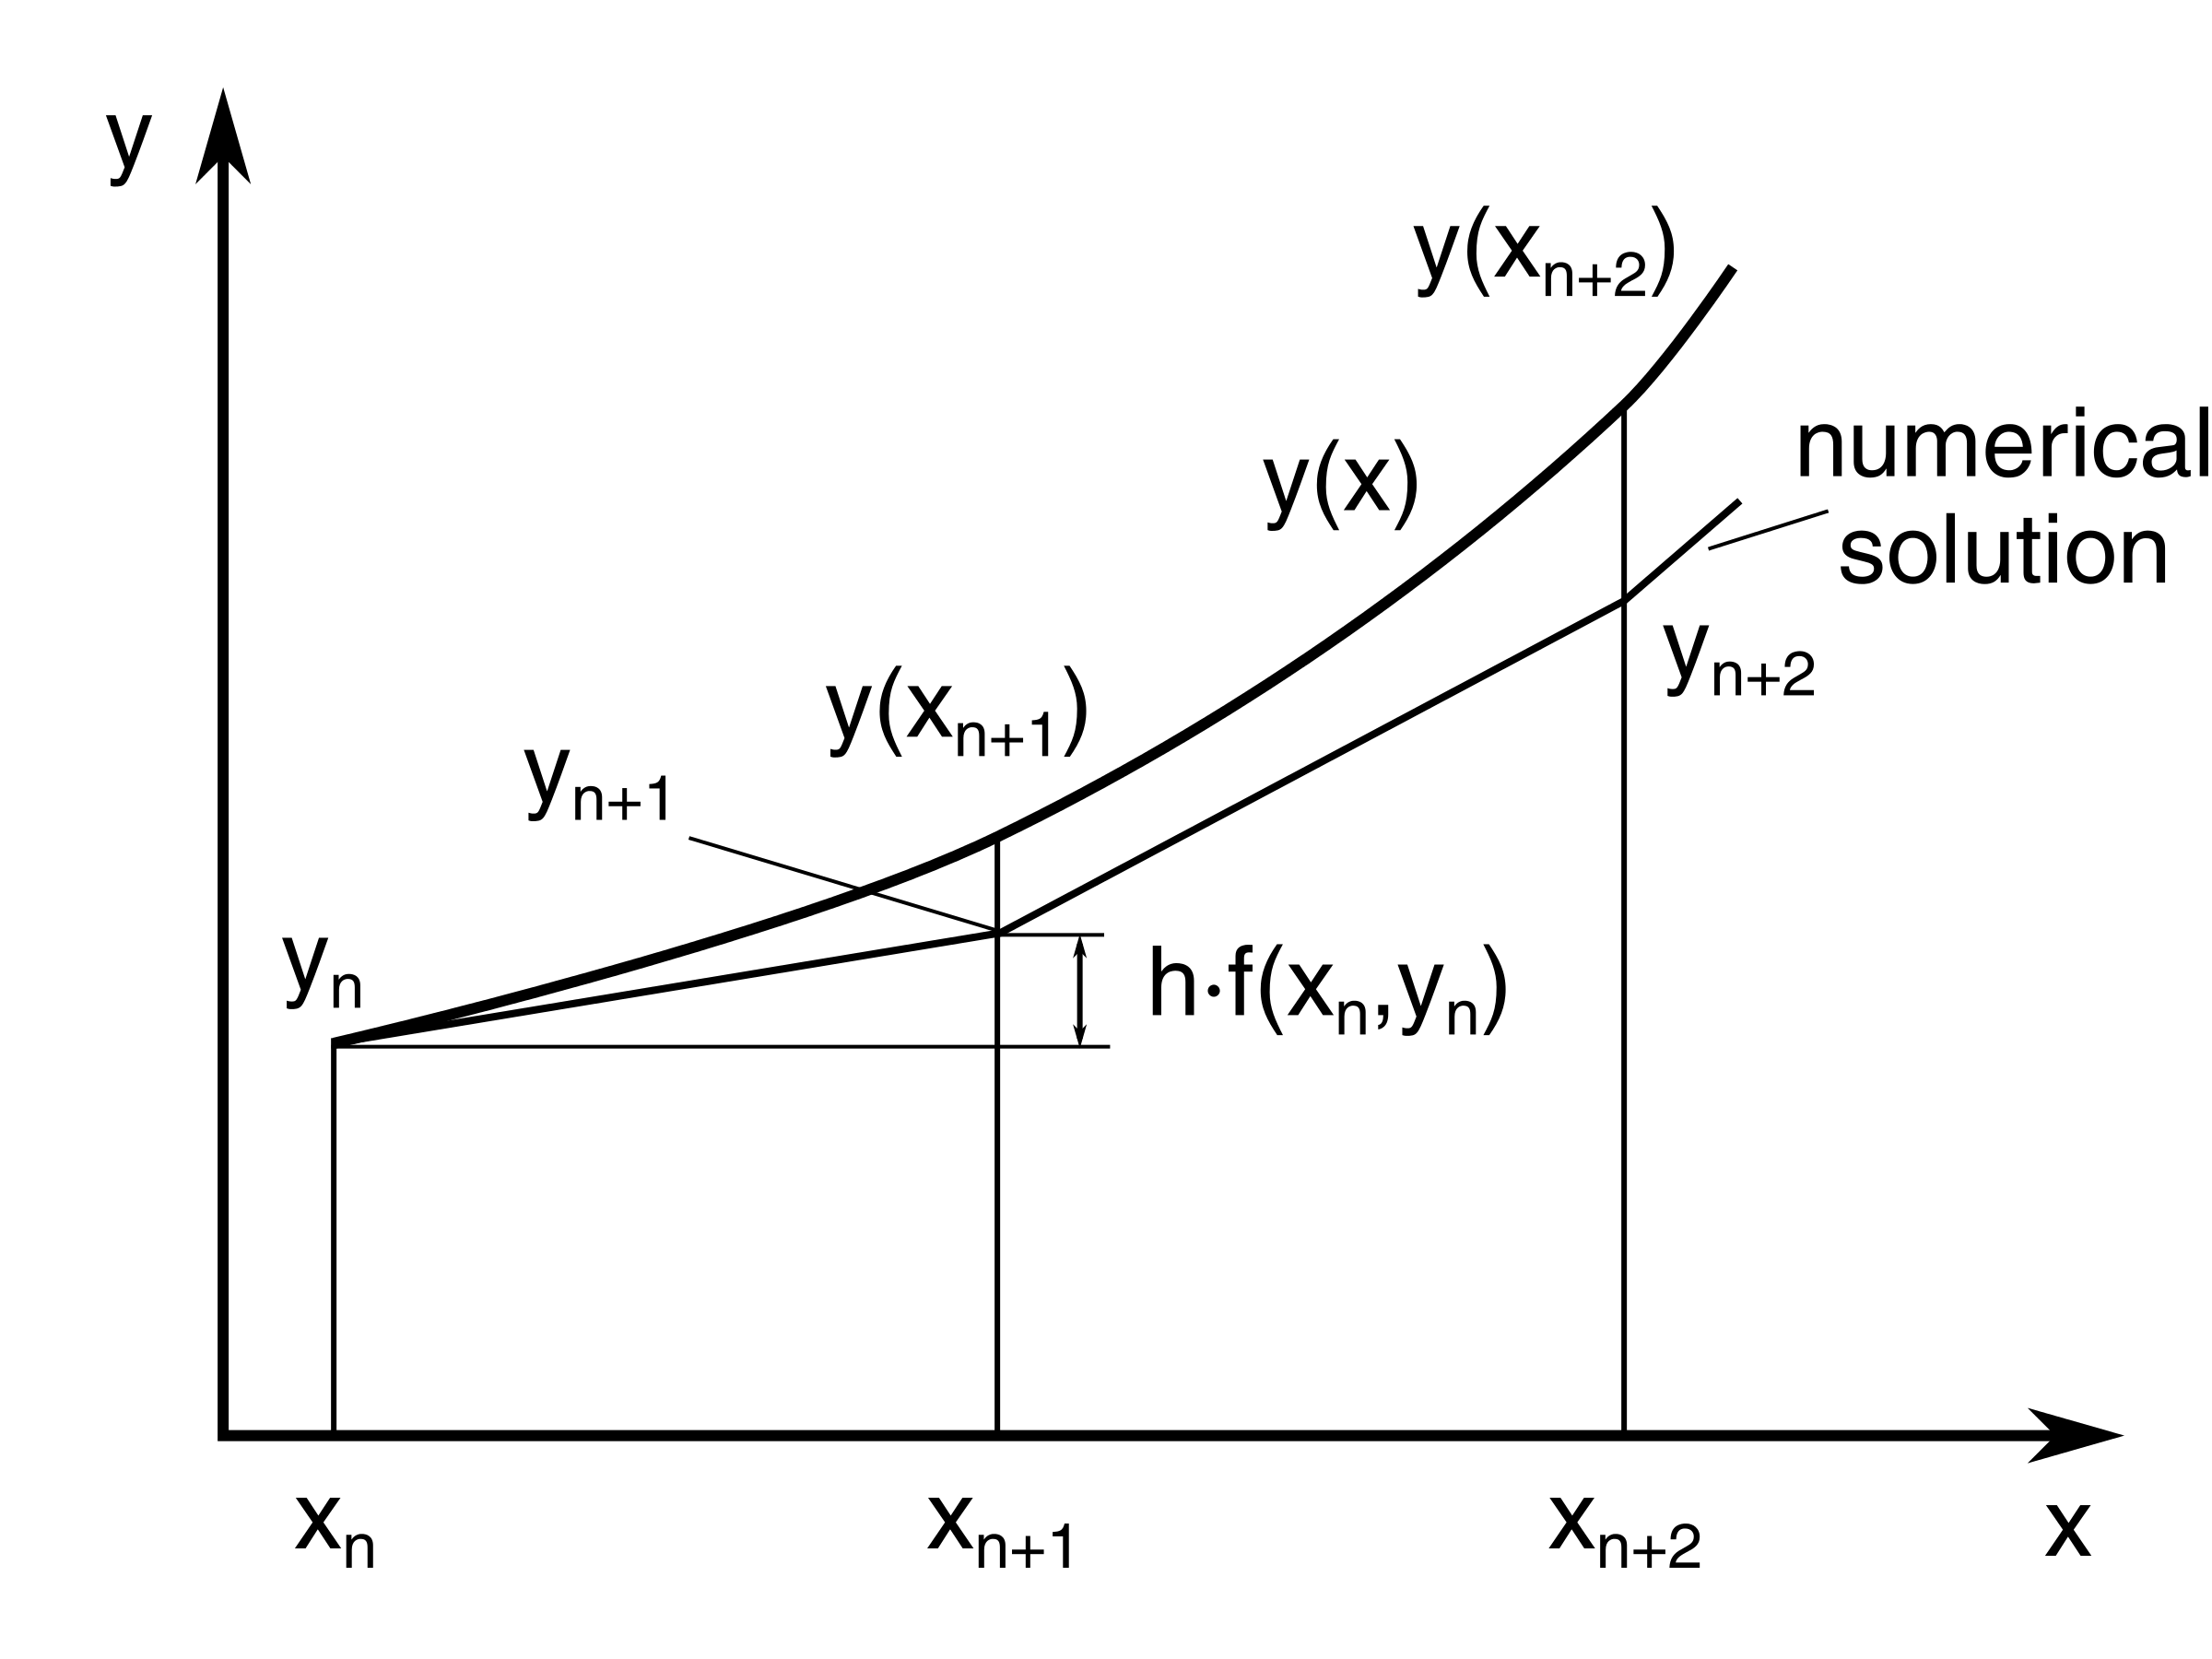
\includegraphics[width=0.90\textwidth]{img/Euler.png}
    \caption{Euler's method schematic}
    \label{fig:euler-png}
\end{figure}

In Euler's method, you can approximate the curve of the solution byt the tangent
in each interval (that is, by a sequence of shor line segments), at steps of $ h $.

\textit{In general}, if you use small step size, the accuracy of the approximation
increases.

\textbf{General Formula}

\begin{equation}
    y_{i+1} = y_i + h f(x_i,y_i)
\end{equation}

where:\\
$ y_{i+1} $ is the next estimated solution value,\\
$ y_i $ is the current value,\\
$ h $ is the interval between steps and\\
$ f(x_i,y_i) $ is the value of the derivative at the current $ (x_i,y_i) $ point.

\textbf{Pseudocode:}

\begin{itemize}
    \item define: $ f(x,y) $

    \item input: $ x_0 $, $ y_0 $

    \item input: $ h $, $ n $

    \item for $ j $ from $ 0 $ to $ (n-1) $ do
        \begin{itemize}
            \item $ y_{j+1} = y_j + hf(x_j, y_j) $
            \item $ x_{j+1} = x_j + h $
            \item Print $ x_{j+1} $ and $= y_{j+1} $
        \end{itemize}
    \item End.
\end{itemize}


\begin{bbox}[0.96]
\textbf{Note:}

If thinking about a problem in time domain:

\begin{itemize}
    \item define: $ f(t,x) $

    \item input: $ t_0 $, $ x_0 $

    \item input: $ dt $, $ n $

    \item for $ j $ from $ 0 $ to $ (n-1) $ do
        \begin{itemize}
            \item $ x_{j+1} = x_j + dt f(t_j, x_j) $
            \item $ t_{j+1} = t_j + dt $
            \item Print $ t_{j+1} $ and $= x_{j+1} $
        \end{itemize}
    \item end.
\end{itemize}

\end{bbox}


\newpage
\textbf{Python Code for vibration problem:}

\begin{python}
#!/usr/bin/python3
import numpy as np
import matplotlib.pyplot as plt


def iterate(h, y0, func, rhs):
    num_of_odes = y0.shape[0]
    y1 = np.zeros(num_of_odes, dtype = float)
    for i in range(num_of_odes-1):
        y1[i] = y0[i] + y0[i+1] * h
    y1[-1] = func(y1, rhs)
    return y1


def euler(t, y, func, rhs):
    N = t.shape[0]
    for j in range(N-1):
        dt = t[j+1] - t[j]
        y[j+1,:] = iterate(dt, y[j,:], func, rhs[j])
        # print(y[j+1,:])
    return y


def euler_vibration():
    m = 0.55  # tonnes
    c = 3.    # Ns/mm
    k = 1000. # N/mm

    freq = np.sqrt(k / m) / (2 * np.pi)

    # equation to solve
    # m * a + c * v + k * u = f
    # a = (f - c * v - k * u) / m
    acceleration = lambda u, f: (f - c * u[1] - k * u[0]) / m

    T = 2.0     # seconds
    dt = 0.0001 # timestep s
    u_0 = 0.    # mm of initial displacement
    v_0 = 0.    # mm/s of initial velocity

    # times at which to solve
    t = np.linspace(0, T, int(T/dt) + 1)

    # force vector
    F = 5000. # N of max impulse
    t0 = 0.1  # impulse start time
    t1 = 0.2  # impuls end time
    f = np.zeros(t.shape[0], dtype=float)
    # create a half sine impulse of force
    for i in range(t.shape[0]):
        if t[i] >= t0 and t[i] <= t1:
            f[i] = F * np.sin((t[i] - t0) / (t1 - t0) * np.pi)
        else:
            f[i] = 0.

    uva = np.zeros((t.shape[0],3), dtype=float)
    uva[0,0] = u_0
    uva[0,1] = v_0

    uva = euler(t, uva, acceleration, f)

    fig, axf = plt.subplots()
    fig.subplots_adjust(right=0.60)

    p1, = axf.plot(t, f, label='force', color='violet')
    axu = axf.twinx()
    p2, = axu.plot(t, uva[:,0], label='displacement', color='red')
    axv = axf.twinx()
    axv.spines.right.set_position(('axes', 1.20))
    p3, = axv.plot(t, uva[:,1], label='velocity', color='blue')
    axa = axf.twinx()
    axa.spines.right.set_position(('axes', 1.40))
    p4, = axa.plot(t, uva[:,2], label='acceleration', color='green')

    axf.set_xlabel('Time [s]')
    axf.set_ylabel('Force [N]')
    axu.set_ylabel('Displacement [mm]')
    axv.set_ylabel('Velocity [mm/s]')
    axa.set_ylabel('Acceleration [mm/s2]')

    axf.legend(handles=[p1, p2, p3, p4])

    plt.show()

if __name__ == '__main__':
    euler_vibration()

\end{python}

Which results to:
\begin{figure}[ht]
    \centering
    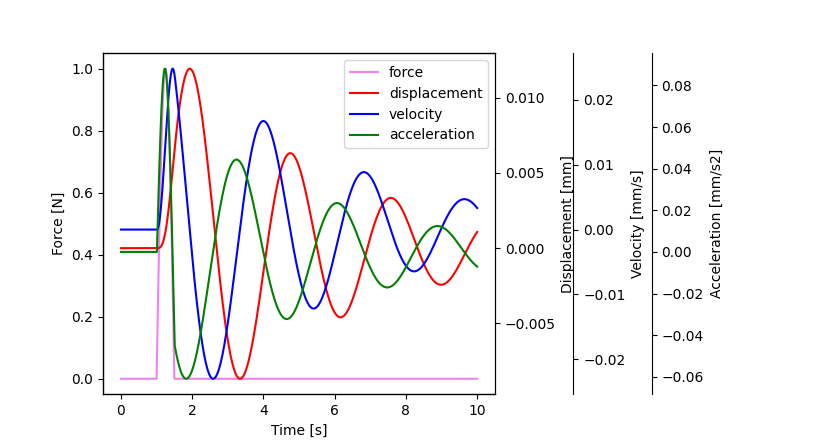
\includegraphics[width=0.90\textwidth]{img/euler_example.png}
    \caption{Euler's implementation for vibration problem example}
    \label{fig:euler-example-png}
\end{figure}


The \textbf{iterate()} function:
\begin{python}
def iterate(h, y0, func, rhs):
    num_of_odes = y0.shape[0]
    y1 = np.zeros(num_of_odes, dtype = float)
    for i in range(num_of_odes-1):
        y1[i] = y0[i] + y0[i+1] * h
    y1[-1] = func(y1, rhs)
    return y1

\end{python}

is written for general case of a set of ODEs. When considering the problem
of vibration (set of 2 ODEs):
\begin{python}
def iterate(h, u0, v0, a0, f, m , c, k):
    u1 = u0 + h * v0
    v1 = v0 + h * a0
    # m * a + c * v + k * u = f
    a1 = (f - c * v1 - k * u1) / m
    return np.array([u1, v1, a1], dtype=float)
\end{python}

which is the iteration of a set of \textbf{first order ODEs}:
\begin{eqarray}
    v &= \dot{u}\\
    \dot{v} &= \frac{f - c * v - k * u}{m}
\end{eqarray}


\newpage
\subsection{Runge-Kutta 4th order method}

\textbf{Runge-Kutta 4th order method} is another explicit method for solving
\textbf{first order ODEs}. The basic equation is:

\begin{equation}
    \frac{dy}{dx} = f(x,y) \quad , y(0) = y_0
\end{equation}

The formula for the next value $ y_{i+1} $ after a step size equal to $h $ is given by:

\begin{eqarray}
    k_1 &= h f(x_i, y_i)\\
    k_2 &= h f(x_i + \frac{h}{2}, y_i + \frac{k_1}{2})\\
    k_3 &= h f(x_i + \frac{h}{2}, y_i + \frac{k_2}{2})\\
    k_4 &= h f(x_i + h, y_i + k_3)\\
    y_{i+1} &= y_i + \frac{k_1}{6} + \frac{k_2}{3} + \frac{k_3}{3} + \frac{k_4}{6} + O(h^5)
\end{eqarray}

The formula basically computes next value $ y_{i+1} $ using current $ y_i $ plus
\textbf{weighted average of four increments}:

\begin{itemize}
    \item $ k_1 $ is the increment based on the slope at the beginning of the
    interval, using $ y $

    \item $ k_2 $ is the increment based on the slope at the midpoint of the interval,
        using $ y + h k_1 / 2 $

    \item $ k_3 $ is the increment based on the slope at the midpoint,
        using $ y + h k_2 / 2 $

    \item $ k_4 $ is the increment based on the slope at the end of the interval,
        using $ y + h k_3 / 2 $

\end{itemize}

The method is a fourth order method, meaning that the local truncation error is
on the order of $ O(h^5) $, while the total accumulated error is of order $ O(h^4) $.

\begin{figure}[ht]
    \centering
    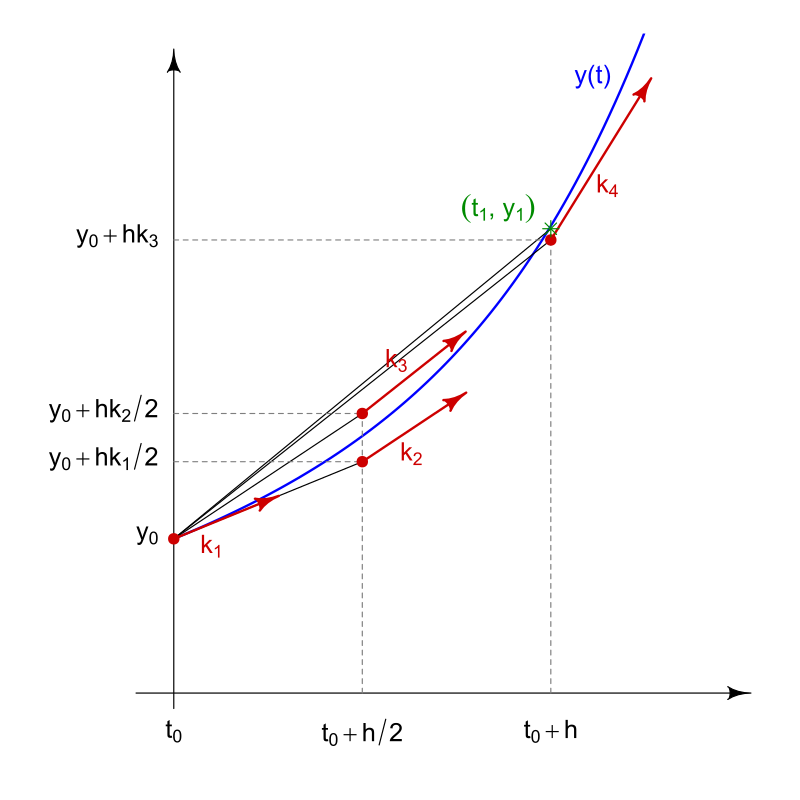
\includegraphics[width=0.80\textwidth]{img/Runge-Kutta_slopes.png}
    \caption{4th Order Runge-Kutta's method schematic}
    \label{fig:rk4-schema-png}
\end{figure}

\newpage
\begin{bbox}[0.96]
\textbf{Note:}

The formula for the next value $ y_{i+1} $ can be also written as:

\begin{eqarray}
    k_1 &= y_i\\
    k_2 &= y_i + \frac{h}{2} \frac{d k_1}{dx}\\
    k_3 &= y_i + \frac{h}{2} \frac{d k_2}{dx}\\
    k_4 &= y_i + h \frac{k_3}{dx}\\
    y_{i+1} &= y_i + \frac{h}{6} (\frac{d k_1}{dx} + 2 \frac{d k_2}{dx}
                              + 2 \frac{d k_3}{dx} + \frac{d k_4}{dx}) + O(h^5)
\end{eqarray}
\end{bbox}

\begin{bbox}[0.96]
This notation is more convenient to use when solving sets of ODEs for vibration
problem, because it translates to:

\begin{eqarray}
    u_1 &= u_0\\
    v_1 &= v_0\\
    a_1 &= (f - c v_0 - k u_0) / m\\
    u_2 &= u_0 + \frac{h}{2} v_1\\
    v_2 &= v_0 + \frac{h}{2} a_1\\
    a_2 &= (f - c v_1 - k u_1) / m\\
    u_3 &= u_0 + \frac{h}{2} v_2\\
    v_3 &= v_0 + \frac{h}{2} a_2\\
    a_3 &= (f - c v_2 - k u_2) / m\\
    u_4 &= u_0 + h v_3\\
    v_4 &= v_0 + h a_3\\
    a_4 &= (f - c v_3 - k u_3) / m\\
    u_{i+1} &= u_0 + \frac{h}{6} \left( v_1 + 2 v_2 + 2 v_3 + v_4 \right) \\
    v_{i+1} &= v_0 + \frac{h}{6} \left( a_1 + 2 a_2 + 2 a_3 + a_4 \right) \\
    a_{i+1} &= (f - c v_{i+1} - k u_{i+1}) / m\\
\end{eqarray}

where each of the \textbf{ODEs} are solved sequentially from the values
already known.

\end{bbox}

\newpage
\textbf{Python implementation for vibration problem:}

\begin{python}
#!/usr/bin/python3
import numpy as np
import matplotlib.pyplot as plt


def iterate(h, y0, y, func, rhs):
    num_of_odes = y0.shape[0]
    y1 = np.zeros(num_of_odes, dtype = float)
    for i in range(num_of_odes-1):
        y1[i] = y0[i] + y[i+1] * h
    y1[-1] = func(y1, rhs)
    return y1


def runge_kutta_4(t, y, func, rhs):
    N = t.shape[0]
    for j in range(N-1):
        dt = t[j+1] - t[j]
        y1 = iterate(0., y[j,:], y[j,:], func, rhs[j])
        y2 = iterate(dt/2, y[j,:], y1, func, 0.5 * (rhs[j+1] + rhs[j]))
        y3 = iterate(dt/2, y[j,:], y2, func, 0.5 * (rhs[j+1] + rhs[j]))
        y4 = iterate(dt, y[j,:], y3, func, rhs[j+1])

        # next step solution
        for i in range(y.shape[1]-1):
            y[j+1,i] = y[j,i] + dt/6 * (y1[i+1] + 2 * y2[i+1] + 2 * y3[i+1] + y4[i+1])
        y[j+1,-1] = func(y[j+1,:], rhs[j+1])
    return y


def rk4_vibration():
    m = 10.   # tonnes
    c = 5.    # Ns/mm
    k = 50.   # N/mm

    freq = np.sqrt(k / m) / (2 * np.pi)
    print(f'f = {freq}')

    # equation to solve
    # m * a + c * v + k * u = f
    # a = (f - c * v - k * u) / m
    acceleration = lambda u, f: (f - c * u[1] - k * u[0]) / m

    T = 10.     # seconds
    dt = 0.01   # timestep s
    u_0 = 0.    # mm of initial displacement
    v_0 = 0.    # mm/s of initial velocity

    # times at which to solve
    t = np.linspace(0, T, int(T/dt) + 1)

    # force vector
    F = 1.    # N of max impulse
    t0 = 1.   # impulse start time
    t1 = 1.5  # impuls end time
    f = np.zeros(t.shape[0], dtype=float)
    # create a half sine impulse of force
    for i in range(t.shape[0]):
        if t[i] >= t0 and t[i] <= t1:
            f[i] = F * np.sin((t[i] - t0) / (t1 - t0) * np.pi)
        else:
            f[i] = 0.

    uva = np.zeros((t.shape[0],3), dtype=float)
    uva[0,0] = u_0
    uva[0,1] = v_0

    uva = runge_kutta_4(t, uva, acceleration, f)

    fig, axf = plt.subplots()
    fig.subplots_adjust(right=0.60)

    p1, = axf.plot(t, f, label='force', color='violet')
    axu = axf.twinx()
    p2, = axu.plot(t, uva[:,0], label='displacement', color='red')
    axv = axf.twinx()
    axv.spines.right.set_position(('axes', 1.20))
    p3, = axv.plot(t, uva[:,1], label='velocity', color='blue')
    axa = axf.twinx()
    axa.spines.right.set_position(('axes', 1.40))
    p4, = axa.plot(t, uva[:,2], label='acceleration', color='green')

    axf.set_xlabel('Time [s]')
    axf.set_ylabel('Force [N]')
    axu.set_ylabel('Displacement [mm]')
    axv.set_ylabel('Velocity [mm/s]')
    axa.set_ylabel('Acceleration [mm/s2]')

    axf.legend(handles=[p1, p2, p3, p4])

    plt.show()

if __name__ == '__main__':
    rk4_vibration()

\end{python}

Which results to:
\begin{figure}[ht]
    \centering
    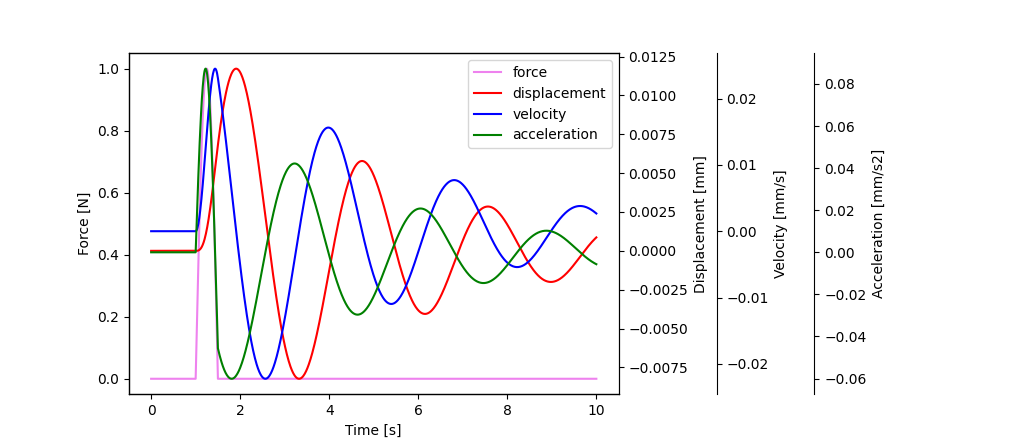
\includegraphics[width=0.90\textwidth]{img/rk4_example.png}
    \caption{4th order Runge-Kutta's implementation for vibration problem example}
    \label{fig:rk4-example-png}
\end{figure}



\newpage
\section{Implicit}

The basic approach is an incremental step-by-step solution with an assumtion
that the solution for a discrete time $ t $ is known and that the solution for
the discrete time $ t + \Delta t $ is required, where $ \Delta t $ is
a suitably chosen time increment. Hence, considering time $ t + \Delta t $:

\begin{equation}\label{implicit-equation}
    \m{F}^{t + \Delta t} - \m{N}^{t + \Delta t} = \m{0}
\end{equation}

Where $ \m{F} $ is the vector of external forces (loads) and $ \m{N} $
is the vector of inner forces.

Assume that $ \m{F}^{t + \Delta t} $ is independent of the deformations.
Since the solution is known at time $ t $, we can write:

\begin{equation}
    \m{N}^{t+\Delta t} = \m{N}^t + \Delta \m{N}
\end{equation}

where $ \Delta \m{N} $ is the increment in nodal point forces corresponding
to the increment in element displacements and stresses from time $ t $ to time
$ t + \Delta t $. This vector can be approximated using a \textbf{tangent stiffness matrix}
$ \m{K}^t $ which corresponds to the geometric and material conditions
at time $ t $,

\begin{equation}\label{internal-forces-approximation}
    \Delta \m{N} \doteq \m{K}^{t} \Delta \m{u}
\end{equation}

where $ \Delta \m{u} $ is a vector of incremental nodal point displacements and

\begin{equation}\label{tangent-stiffness-matrix}
    \m{K}^{t} = \frac{\partial \m{N}^{t}}{\partial \m{u}^{t}}
\end{equation}

Hence, the \textbf{tangent stiffness matrix} corresponds to the derivative of the
internal element nodal point forces $ \m{N}^{t} $ with respect to the
nodal point displacements $ \m{u}^{t} $.

Substituting \eqref{internal-forces-approximation} and
\eqref{tangent-stiffness-matrix} into \eqref{implicit-equation}, we obtain

\begin{equation}\label{iteration-equation}
    \m{K}^{t} \Delta \m{u} = \m{F}^{t + \Delta t} - \m{N}^{t}
\end{equation}

and solving for $ \m{u}^{\Delta t} $, we can calculate and approximation
to the displacements at time $ t + \Delta t $,

\begin{equation}\label{iteration-displacements}
    \m{u}^{t + \Delta t} \doteq \m{u}^{t} + \Delta \m{u}
\end{equation}

The exact displacements at time $ t + \Delta t $ are those that correspond to the
applied loads $ \m{F}^{t + \Delta t} $. We calculate in \eqref{iteration-displacements}
only an approximation to these displacements because \eqref{internal-forces-approximation}
was used.

Having evaluated an approximation to the displacements corresponding to
time $ t + \Delta t $, we could now solve for an approximation to the stresses and
corresponding nodal point forces at time $ t + \Delta t $, and then proceed to the
next time increment calculations. However, because of the assumption
\eqref{internal-forces-approximation}, such a solution may be subject to
very significant errors and, depending on the time or load step sizes used, may
indeed be unstable. In practice, it is therefore necessary to iterate until the
solution of \eqref{implicit-equation} is obtained to sufficient accuracy.


\subsection{Newton-Raphson}
Having calculated an \textit{increment} in nodal point displacements, which defines
a \textit{new total} displacement vector, we can repeat ht incremental solution
using the currently known total displacements at time $ t $.

The equations used in \textbf{Newton-Raphson} iteration are, $ for\ i = 1, 2, 3, \dots, $

\begin{bbox}
    \begin{eqarray}\label{newton-raphson}
        \m{K}_{i-1}^{t + \Delta t} \Delta \m{u}_i &=
        \m{F}^{t + \Delta t} - \m{N}_{i - 1}^{t + \Delta t} \\
        \m{u}_{i}^{t+\Delta t} &=  \m{u}_{i}^{t + \Delta t} +
        \m{u}_{i-1}^{t+\Delta t} + \Delta \m{u}_i
    \end{eqarray}
\end{bbox}

with the initial conditions:

\begin{eqarray}
    \m{u}_{0}^{t + \Delta t} &= \m{u}^t \\
    \m{K}_{0}^{t + \Delta t} &= \m{K}^t \\
    \m{N}_{0}^{t + \Delta t} &= \m{N}^t \\
\end{eqarray}

Note that in the first iteration, the relations in \eqref{newton-raphson}
reduce to the equations \eqref{iteration-equation} and \eqref{iteration-displacements}.
Then, in subsequent iterations, the latest estimates for the nodal point
displacements are used to evaluate the corresponding element stresses and
nodal point forces $ \m{N}_{i-1}^{t + \Delta t} $ and
\textbf{tangent stiffness matrix} $ \m{K}_{i-1}^{t + \Delta t} $.

The out-of-balance load vector $ \m{F}^{t + \Delta t} - \m{N}_{i-1}^{t + \Delta t} $
corresponds to a load vector that is not yet balanced by element stress, and
hence an increment in the nodal point displacement is required. This updating of the
nodal point displacement in the iteration is continued until out-of-balance loads
and incremental displacements are small enough.

An important point is that the calculation of $ \m{N}_{i-1}^{t + \Delta t} $
from $ \m{u}_{i-1}^{t + \Delta t} $ is \textbf{crucial}. Any errors in this
calculation will, in general, result in an incorrect response prediction.

The correct evaluation of the \textbf{tangent stiffness matrix}
$ \m{K}_{i-1}^{t + \Delta t} $ is also important. The use of proper
\textbf{tangent stiffness matrix} may be necessary for convergence and, in general,
will result in fewer iterations until convergence is reached.

However, because the expense involved in evaluating and factoring a new
\textbf{tangent stiffness matrix}, in practice, it can be more efficient,
depending on the nonlinearities present in the analysis, to evaluate a new
\textbf{tangent stiffness matrix} only at certain times. Specifically,
in the \textbf{modified Newton-Raphson method} a new \textbf{tangent stiffness matrix}
is established only at the beginning of each load step, and in
\textbf{quasi-Newton} methods \textbf{secant stiffness matrices} are used
instead of the tangent stiffness matrix.

The use of the iterative solution requires appropriate convergence criteria.
If inappropriate criteria are used, the iteration may be terminated before
the necessary solution accuracy is reached or be continued after the required
accuracy has been reached.

\subsubsection{Full Newton-Raphson Procedure derivation}

The finite element equilibrium requirements amount to finding the solution
of the equations:

\begin{equation}\label{nr-error}
    f( \m{u}^* ) = 0
\end{equation}

Where:

\begin{equation}\label{nr-error-expanded}
    f( \m{u}^* ) = \m{F}^{t + \Delta t} ( \m{u}^* )
    - \m{N}^{t + \Delta t} ( \m{u}^* )
\end{equation}

We denote here and in the following the complete array of the solution as
$ \m{u}^* $ but realize that this vector may also contain variables other
than displacements, for example, pressure variables and rotations.

Assume that in the iterative solution we have evaluated $ \m{u}_{i-1}^{t + \Delta t} $;
then a Taylor series expansion gives:

\begin{eqarray}\label{newton-raphson-taylor-expansion}
    f(\m{u}^*) &= f(\m{u}_{i-1}^{t + \Delta t})
    + \left. \left[\frac{\partial N}{\partial \m{u}} \right]
        \right|_{\m{u}_{i-1}^{t + \Delta t}}
        \left( \m{u}^* - \m{u}_{i-1}^{t + \Delta t} \right) \\
                    &+ higher\ order\ terms
\end{eqarray}

Substituting from \eqref{nr-error-expanded} into \eqref{newton-raphson-taylor-expansion}
and using \eqref{nr-error}, we obtain:

\begin{eqarray}\label{nr-taylor}
    & \left. \left[ \frac{\partial \m{N}}{\partial \m{u}} \right]
        \right|_{\m{u}_{i-1}^{t + \Delta t}}
    \left(\m{u}^* - \m{u}_{i-1}^{t + \Delta t} \right)
    + higher\ order\ terms\\
    & = \m{F}^{t + \Delta t} - \m{N}_{i-1}^{t + \Delta t}
\end{eqarray}

where we assumed that the externally applied loads are deformation independent.

Neglecting the higher-order terms in \eqref{nr-taylor}, we can calculate an increment
in the displacements,

\begin{equation}\label{nr-displacement-increment}
    \m{K}_{i-1}^{t + \Delta t} \Delta \m{u}_i =
    \m{F}^{t + \Delta t} - \m{N}_{i-1}^{t + \Delta t}
\end{equation}

where $ \m{K}_{i-1}^{t + \Delta t} $ is the current \textbf{tangent stiffness matrix}

\begin{equation}
     \m{K}_{i-1}^{t + \Delta t} =
     \left. \left[ \frac{\partial \m{N}}{\partial \m{u}} \right]
        \right|_{\m{u}_{i-1}^{t + \Delta t}}
\end{equation}

and the improved displacement solution is:

\begin{equation}\label{nr-displacement}
    \m{u}_i^{t + \Delta t} =
    \m{u}_{i-1}^{t + \Delta t} +
    \Delta \m{u}_{i}
\end{equation}

\textit{The relations in} \eqref{nr-displacement-increment} \textit{and} \eqref{nr-displacement}
\textit{costitute the Newton-Raphson solution of} \eqref{implicit-equation}.
Since an incremental analysis is performed with time (or load) steps of size
$ \Delta t $, the initial conditions in this iteration are
$ \m{K}_0^{t + \Delta t} = \m{K}^t $,
$ \m{N}_0^{t + \Delta t} = \m{N}^t $, and
$ \m{u}_0^{t + \Delta t} = \m{u}^t $.
The iteration is continued \textbf{until appropriate convergence criteria are satisfied.}

A characteristic of this iteration is that a new tangent stiffness matrix is
calculated in \textbf{each} iteration, which is why this method is also referred
to as the \textbf{full Newton-Raphson method}.

\begin{figure}[ht]
    \centering
    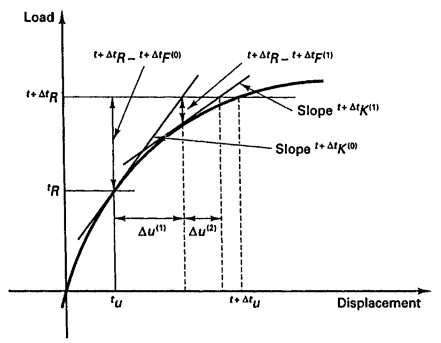
\includegraphics[width=0.60\textwidth]{img/full_newton_raphson.png}
    \caption{Newton-Raphson iteration in solution of SDOF system.
    $ \m{R} $ is load increment, $ \m{F} $ are internal forces,
    $ \m{u} $ are displacements.}
    \label{fig:full-newton-raphson-png}
\end{figure}

% TODO: Bathe FEP_2nd_Edidtion_4th_prinitng.pdf
%       Page 756 (773)
%       Modified Newton-Raphson

